\documentclass[10pt,a4paper]{article}
\usepackage{fullpage}
\usepackage{graphicx}
\usepackage{fancyhdr}
\setlength{\headheight}{13pt}
\pagestyle{fancy}

% default sans-serif
\renewcommand{\familydefault}{\sfdefault}

% no lines for headers and footers
\renewcommand{\headrulewidth}{0pt}
\renewcommand{\footrulewidth}{0pt}

% header
\fancyhf{}
\lhead{GWD-R}
\rhead{\today}

% footer
\lfoot{occi-wg@ogf.org}
\rfoot{\thepage}

% paragraphs need some space...
\setlength{\parindent}{0pt}
\setlength{\parskip}{1ex plus 0.5ex minus 0.2ex}

% some space between header and text...
\headsep 13pt

\setcounter{secnumdepth}{4}

\begin{document}

% header on first page is different
\thispagestyle{empty}

GWD-R \hfill Thijs Metsch, Platform Computing\\
OCCI-WG \hfill Andy Edmonds, Intel\\
\rightline {October 7, 2010}\\
\rightline {Updated: \today}

\vspace*{0.5in}

\begin{Large}
\textbf{Open Cloud Computing Interface - HTTP Rendering}
\end{Large}

\vspace*{0.5in}

\underline{Status of this Document}

This document provides information to the community regarding the specification of the Open Cloud Computing Interface. Distribution is unlimited.

\underline{Obsoletes}

This document obsoletes GFD-xxx [REFERENCE].

\underline{Copyright Notice}

Copyright \copyright Open Grid Forum (2009-2010). All Rights Reserved.

\underline{Trademarks}

OCCI is a trademark of the Open Grid Forum.

\underline{Abstract}

This document, part of a document series, produced by the OCCI working group within the Open Grid Forum (OGF), provides a high-level definition of a Protocol and API. The document is based upon previously gathered requirements and focuses on the scope of important capabilities required to support modern service offerings. 

\newpage
\tableofcontents
\newpage

\section{Introduction}

The Open Cloud Computing Interface (OCCI) is a RESTful Protocol (and API) for all kinds of Management tasks. Originally initiated to create a remote management API for IaaS model based Services, allowing for the development of interoperable tools for common tasks including deployment, autonomic scaling and monitoring, it now can be used to severe other models as well. To be modular and extensible the current specification itself is currently split into three complimentary documents:

\begin{itemize}
\item Core – this defines the OCCI model
\item HTTP Rendering - this defines how to manipulate the core model using the OCCI RESTful API. The document defines how the OCCI model can be communicated and thus serialized using HTTP.
\item Infrastructure – this defines the infrastructure domain resource types, the required attributes for each and the actions that can be taken on each.
\end{itemize}

\section{Notational Conventions}

All these parts and the information within are mandatory for implementors (unless otherwise specified). The key words "MUST", "MUST NOT", "REQUIRED", "SHALL", "SHALL NOT", "SHOULD", "SHOULD NOT", "RECOMMENDED", "MAY", and "OPTIONAL" in this document are to be interpreted as described in RFC 2119. 

UML activity diagrams do not specify how OCCI should be rendered but what possible request and outcomes can be.

\section{HTTP Rendering}
The HTTP Protocol is the underlying core fabric of OCCI and uses all the features of the HTTP and underlying protocols (like self-healing capabilities of TCP) offer. OCCI also builds upon the Resource Oriented Architecture (ROA). ROA's use Representation State Transfer (REST) to cater for client and service interactions. Interaction with the system is by inspection and modification of a set of related resources and their states, be it on the complete state or a sub-set. Resources must be uniquely identified. HTTP is an ideal protocol to use in ROA systems as it provides the means to uniquely identify individual resources through URLs as well as operating upon them with a set of general-purpose HTTP verbs. These HTTP verbs map loosely to the resource related operations of Create (POST), Retrieve (GET), Update (POST/PUT) and Delete (DELETE).

The following notations are used when referring to parts or complete URIs:

\begin{verbatim}
http://www.example.com:8080/foo/bar;action=stop
<   >  <     Authority    >< Path >< Fragment >
  ^
  Scheme
\end{verbatim}

The following section describe the general behavior for all HTTP based renderings. Later sections will describe the syntax and semantic of how to render the OCCI Core model with different Content-Types.

\subsection{Identification of Kinds}
Each Kind sub-type instance within an OCCI system must be uniquely identified by an URI. The structure of these URIs is opaque and the system should not assume a static, pre-determined scheme for their structure.

\subsection{Interaction with Kinds}
As OCCI adopts a ROA, REST-based architecture and uses HTTP as the foundation protocol the means of interaction with all RESTful resource instances is through the four main HTTP verbs. OCCI service implementations must, at a minimum, support these verbs:

\begin{tabular}{l|p{3.2in}|p{2in}}
Verb & RFC Definition & Usage in OCCI context \\
\hline
POST & The POST method is used to request that the origin server accept the resource enclosed in the request as a new subordinate of the resource identified by the Request-URI in the Request- Line & This is the verb will be used when creating Kinds. POST can also be used to create a sub-resource of an existing resource type. Action are also triggered using the POST verb. \\
GET & The GET method means retrieve whatever information (in the form of a resource) is identified by the Request-URI & Retrieving one Kind or Category using GET will result in a representation of the resource. Lists of Kinds and Categories are also retrieved through GET (Discovery/Querying). \\
PUT & The PUT method requests that the enclosed resource be stored under the supplied Request-URI & The PUT verb will be used when updating a Kind or when creating an Kind at a specific location\footnote{In difference to POST where sub-resources will be created}. \\
DELETE & The DELETE method requests that the origin server delete the resource identified by the Request-URI & This verb is used to destroy instances of Kinds. \\ 
\end{tabular}

\subsection{Security and Authentication}
OCCI does not require that an authentication mechanism be used nor does it require that client to service communications are secured. It does recommend that an authentication mechanism be used and that where appropriate, communications are encrypted using HTTP over TLS. The authentication mechanisms that CAN be used with OCCI are those that can be used with HTTP and TLS, for example Basic [REF], Digest [REF] and OAuth [REF]. If an OCCI service requires authentication the response to a request that MUST be authenticated must be a HTTP 401 code that indicates the request is authorized. In response to authenticate the client MUST set a WWW-Authenticate header field and through this indicate the authentication mechanism. 

\subsection{Versioning}
Information about what version of OCCI is supported by a provider MUST be advertised to a client on each response to a client. The version field in the response MUST include the value OCCI/X.Y, where X is the major version number and Y is the minor version number of the implemented OCCI specification. In the case of a HTTP Header Rendering, the server response should relay versioning information using the HTTP header name 'Server'.

\begin{verbatim}
HTTP/1.1 202 Accepted
Server: occi-server/1.1 (linux) OCCI/1.0
[...]
\end{verbatim}

Complimenting the service-side behavior of an OCCI implementation, a client MUST indicate to the OCCI service implementation the version it expects to interact with. For the clients, the information MUST be advertised in the request it issues. In the case of a HTTP Header Rendering, the client request should relay versioning information in the 'User-Agent' header. The 'User-Agent' field must include the same value (OCCI/X.Y) as specified for the Server HTTP header.

\begin{verbatim}
GET <UDN> HTTP/1.1
Host: example.com
User-Agent: occi-client/1.1 (linux) libcurl/7.19.4 OCCI/1.0
[...]
\end{verbatim}

If a server receives a request from a client that supplies a version number higher than the service supports, the service MUST respond back to the client with an exception indicating that the requested version is not implemented. Where a client implements OCCI using a HTTP transport, the HTTP code 501, not implemented should be used. 

\subsection{Content-type and Accept headers}
A server MUST react according to the Accept header the client provides. If non is given - or \textit{text/occi} is used - the service MUST use the HTTP Header Rendering described in section \ref{sec:http_header}. This is the fall-back rendering and MUST be implemented. Otherwise the according rendering MUST be used. Each Rendering SHOULD expose which Accept and Content-type header fields it can handle. Overall the server MUST support the \textit{text/occi}, \textit{text/plain} and \textit{text/uri-list} Content-types.

The server MUST also return the proper Content-type header. If a client POSTs information with a Content-Type - the information MUST be parsed accordingly.

\subsection{Discovery and Listing}
When performing an GET operation an server MUST reply with a listing of matching Kinds. If the request was preformed on a Path of an URI only the sub-resource SHOULD be returned. If a Category was given in the request the server MUST only give back Kinds which have this Category assigned.

If the request was performed on the \textit{/-/} Path a list of Categories which the server can handle MUST be returned. Categories used for tagging are not exported via this mechanism.

\subsection{Behavior of HTTP operations}

More information on how OCCI compatible Service should handle the HTTP verbs is given in these sections. Possible results are demonstrated here. How to render the results is described later on.

\newpage
\subsubsection{The HTTP POST Operation behavior}

The UML diagram \ref{fig:post_operation} shows what the Server can return, and what it will return when performing an POST operation.

\begin{figure}[!hp]
	\centering
	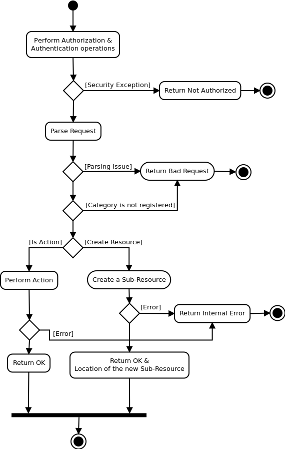
\includegraphics[scale=0.4]{POST_operation.png}
	\caption{Behavior for HTTP POST}
	\label{fig:post_operation}
\end{figure}

The OCCI service implementation MUST create sub resource of and existing URN (which can be Root). Action must be exposed by adding the fragment \emph{;action=$<$action term$>$} to the URI.

\newpage
\subsubsection{The HTTP PUT Operation behavior}

The UML diagram \ref{fig:put_operation} shows what the Server can return, and what it will return when performing an PUT operation. PUT is used to updated Kinds or to create Kinds at certain Paths.

\begin{figure}[!h]
	\centering
	\includegraphics[scale=0.4]{PUT_operation.png}
	\caption{Behavior for HTTP PUT}
	\label{fig:put_operation}
\end{figure}

\newpage
\subsubsection{The HTTP GET Operation behavior}

The UML diagram \ref{fig:get_operation} shows what the Server can return, and what it will return when performing an GET operation. GET is used to return Renderings of Kind, Listings of Kind or for Listing of Categories (Discovery).\footnote{The slashes in the path separate Resource in a hierarchical manner. So a Sub-Resource shares a path with his parent (\textit{http://example.com/foo/bar} is concidered a sub-resource of \textit{http://example.com/foo/})}

\begin{figure}[!h]
	\centering
	\includegraphics[scale=0.4]{GET_operation.png}
	\caption{Behavior for HTTP GET}
	\label{fig:get_operation}
\end{figure}

\newpage
\subsubsection{The HTTP DELETE Operation behavior}

The UML diagram \ref{fig:del_operation} shows what the Server can return, and what it will return when performing an DELETE operation.

\begin{figure}[!h]
	\centering
	\includegraphics[scale=0.4]{DELETE_operation.png}
	\caption{Behavior for HTTP DELETE}
	\label{fig:del_operation}
\end{figure}

\subsection{Render OCCI model in the HTTP Header}
\label{sec:http_header}

\textbf{This Rendering can handle the \textit{text/occi} Accept Header. It will return the same for Content-type}

The HTTP header fields MUST follow the specification in RFC 2616. A header field consists of a name followed by a colon (":") and the field value. The format of the field value is specified separately for each of the three header fields, see below.

HTTP header fields MAY appear multiple times in a HTTP request or response. In order to be OCCI compliant the specification of multiple message-header fields according to RFC 2616 (section 4.2) MUST be fully supported. In essence there are two valid representation of multiple HTTP header field values. A header field might either appear several times or as a single header field with a comma-separated list of field values. Due to implementation issues in many web frameworks and client libraries it is RECOMMENDED to use the comma-separated list format for best interoperability.

HTTP header field values which contain separator characters MUST be properly quoted according to RFC 2616.

\subsubsection{HTTP Header Rendering Caveats}

Space in the HTTP header section of a HTTP request is a limited resource. By this, it is noted that many HTTP servers limit the number of bytes that can be placed in the HTTP Header area. Implementers MUST be aware of this limitation in their own implementation and take appropriate measures so that truncation of header data does NOT occur. 

\emph{TODO: Is further description needed here? Should we show a possible counter-measure in the case where a HTTP header overflow is detected and how it's handled?}
\emph{TODO: Ralf thinks we at least should mention the fallback to text/plain rendering where the relevant headers are just dumped into the body of the response.}

\subsubsection{HTTP Header Fields}

Three different HTTP header fields are used to render the OCCI model. Each header field value has a different format.

\paragraph{Category Header}

The Category header is defined by the Web Categories specification, http://tools.ietf.org/html/draft-johnston-http-category-header-01 and MUST be rendered accordingly. The semantics of the Category header in the OCCI context is described in the OCCI Core \& Models document.
\marginpar{Define ``Categary identifier'' somewhere, i.e. concatenation of scheme + term.}

\begin{verbatim}
Category: <term>; scheme="<scheme>"
    [;rel=<space-separated list of related Category identifiers>]
    [;attributes=<space-seperated list of attribute names>]
    [;title=<Title of this Category>]    
\end{verbatim}

There is NO order for the optional part.

\paragraph{Link Header}

The Link header is defined by the Web Linking specification, http://tools.ietf.org/html/draft-nottingham-http-link-header-10 and MUST be rendered accordingly. The semantics of the Link header in the OCCI context is described in the OCCI Core \& Models document.
\emph{TODO: Link header semantics are NOT described in Core. Link and Action type semantics are described however. How these base types relate to the Link header must be described in this document.}
\marginpar{User proper ABNF grammar to describe the header formats.}

\begin{verbatim}
Link: <Resource URL>;
    rel=<space-separated list of Category identifiers of the target Resource type>
    [;self=<Link instance URL>]
    [;category=<space-separated list of Category identifiers of the Link type>
        [;<attribute name>=<attribute value>] ... ]

or in case it is an Action:

Link: <Resource URL> + ";action=" + <Term of the Action>;
    rel=<Category identifier of the Action>
\end{verbatim}

\paragraph{X-OCCI-Attribute Header}

The X-OCCI-Attribute header MUST be used to render the attributes associated with a OCCI Kind. A simple key-value format is used. The field value consist of an attribute name followed by an equal sign ("=") and the attribute value. The attribute value must be quoted if it includes a separator character, see RFC 2616 (page 16).

\begin{verbatim}
X-OCCI-Attribute: <attribute name>=<attribute value>
\end{verbatim}

Valid attribute names for OCCI Kinds are specified in appropriate Extension documents.

\paragraph{X-OCCI-Location Header}

To render an OCCI representation solely in the header, the X-OCCI-Location header MUST be used to return a list of Kind URLs. Each header field value correspond to a single URL. Multiple Kind URLs are returned using multiple X-OCCI-Location headers. See RFC 2616 for information on how to render multiple HTTP headers.

\begin{verbatim}
X-OCCI-Location: <URL>
\end{verbatim}

\subsubsection{Rendering the OCCI model}

The following setups show how the Core Model MUST be rendered. Shown are the HTTP Header fields which MUST be available in a request from the Client or a response from the Server.

In some cases the framework does not support to have multiple occurrences of one HTTP Header field. If that is the case the server must join the values of the field with a \emph{,} and add this list to one HTTP Header field.

\begin{tabular}{l|l|l|l}
Operation & Required HTTP-Header(s) & Optional HTTP-Header(s) & Notes \\
\hline
Rendering of a Category & Category & N/A & \\
Rendering a list of Categories & Category & N/A & \\
Rendering a list of Kinds & X-OCCI-Location & N/A & \\
Rendering of a Resource & Category & X-OCCI-Attribute, Link & \\
Rendering of an Action & Category, Link & X-OCCI-Attribute & \\
Rendering of a Link & Category, Link & X-OCCI-Attribute & \\
\end{tabular}

\subsection{Render OCCI model in the HTTP Body}
\label{sec:http_body}

\textbf{This Rendering can handle the \textit{text/plain} Accept Header. It will \textit{text/plain} an empty Content-type}

Renderings for this Content-type use the syntax and semantics as those described in section \ref{sec:http_header}. Difference are the following:

\begin{itemize}
  \item The Header fields MUST be placed in the body of HTTP envelope.
  \item On multiple occurrences of an field the field name and it's value MUST be rendered in new lines.
\end{itemize}

\subsubsection{Rendering the OCCI model}

Same behavior MUST be implemented as in section \ref{sec:http_header}.

\subsection{Render OCCI model via URL Listings}

\textbf{This Rendering can handle the \textit{text/uri-list} Accept Header. It will \textit{text/uri-list} an empty Content-type}

This rendering cannot render Kinds or Categories directly but just Links to them. For concrete rendering of Kinds and Categories the Content-types \textit{text/occi}, \textit{text/plain} MUST be used. If a request is done with the \textit{text/uri-list} in the Accept header, while not requesting for a Listing a Bad Request MUST be returned.

\subsubsection{Rendering the OCCI model}

\paragraph{Rendering a list of Categories}

MUST return a list of Category scheme URLs.

\paragraph{Rendering a list of Kinds}

MUST return a list of URLs pointing to the Kinds.

\section{Contributors}

Editors: Andy Edmonds, Thijs Metsch \\
Contributors: Alexander Papaspyrou, Ralf Nyrén, Sam Johnston

\textbf{TBD: Bunch op people missing here - create table\ldots}

\section{Appendix}

\subsection{Examples for rendering the OCCI model in the HTTP Header}

\subsubsection{Creating a Kind}
\begin{verbatim}
> POST / HTTP/1.1
> User-Agent: curl/7.21.0 (x86_64-pc-linux-gnu) libcurl/7.21.0 OpenSSL/0.9.8o zlib/1.2.3.4 libidn/1.18
> Host: localhost:8080
> Accept: */*
> Category:keyvalue;scheme="http://schemas.ogf.org/occi/keyvalue#"
> Attribute:occi.keyvalue.key=foo,occi.keyvalue.value=bar
> Content-Length: 0
> Content-Type: application/x-www-form-urlencoded

< HTTP/1.1 200 OK
< Location: /c815e27f-d0ff-4c59-a0a4-3491ace6d160
< Transfer-Encoding: chunked
< Date: Wed, 13 Oct 2010 10:19:47 GMT
< Server: CherryPy/3.1.2 WSGI Server
< 
< 2
< OK
< 0
\end{verbatim}

\subsubsection{Triggering an Action}

\begin{verbatim}
> POST /624034ee-1448-4fca-81f9-1f4f6a525aa4;action=terminate HTTP/1.1
> User-Agent: curl/7.21.0 (x86_64-pc-linux-gnu) libcurl/7.21.0 OpenSSL/0.9.8o zlib/1.2.3.4 libidn/1.18
> Host: localhost:8080
> Accept: */*
> Category:terminate;scheme="http://schemas.ogf.org/occi/drmaa/action#"

< HTTP/1.1 200 OK
< Transfer-Encoding: chunked
< Date: Mon, 11 Oct 2010 15:27:57 GMT
< Server: CherryPy/3.1.2 WSGI Server
< 
< 2
< OK
< 0
<
\end{verbatim}

\subsubsection{Listing Categories}

\begin{verbatim}
> GET /-/ HTTP/1.1
> User-Agent: curl/7.21.0 (x86_64-pc-linux-gnu) libcurl/7.21.0 OpenSSL/0.9.8o zlib/1.2.3.4 libidn/1.18
> Host: localhost:8080
> Accept: */*

< HTTP/1.1 200 OK
< Category: keyvalue;scheme=http://schemas.ogf.org/occi/keyvalue#;title=A key-value Resource,job;scheme=http://schemas.ogf.org/occi/drmaa#;title=A Job Resource,terminate;scheme=http://schemas.ogf.org/occi/drmaa/action#;title=Terminate a Job
< Transfer-Encoding: chunked
< Date: Wed, 13 Oct 2010 10:15:22 GMT
< Server: CherryPy/3.1.2 WSGI Server
< 
< 4
< None
< 0
\end{verbatim}

\subsubsection{Listing Resources}

\begin{verbatim}
> GET / HTTP/1.1
> User-Agent: curl/7.21.0 (x86_64-pc-linux-gnu) libcurl/7.21.0 OpenSSL/0.9.8o zlib/1.2.3.4 libidn/1.18
> Host: localhost:8080
> Accept: */*

< HTTP/1.1 200 OK
< Location: /4147377d-283d-4947-8696-7c1591e89179
< Transfer-Encoding: chunked
< Date: Mon, 11 Oct 2010 15:11:05 GMT
< Server: CherryPy/3.1.2 WSGI Server
<
< 0
<
\end{verbatim}

\subsubsection{Request with missing Category rendering}

\begin{verbatim}
> PUT /21d0171e-6de3-40ab-b595-25e5de607ccc HTTP/1.1
> User-Agent: curl/7.21.0 (x86_64-pc-linux-gnu) libcurl/7.21.0 OpenSSL/0.9.8o zlib/1.2.3.4 libidn/1.18
> Host: localhost:8080
> Accept: */*

< HTTP/1.1 400 Bad Request
< Content-Type: text/html
< Transfer-Encoding: chunked
< Date: Mon, 11 Oct 2010 15:07:21 GMT
< Server: CherryPy/3.1.2 WSGI Server
< 
< (BadRequest('400 Bad Request',), 'No categories could be found in the header!')
\end{verbatim}

\subsubsection{Retrieving a Kind}

\begin{verbatim}
> GET /bb39bdfc-3e78-44c2-8853-114ba3599d76 HTTP/1.1
> User-Agent: curl/7.21.0 (x86_64-pc-linux-gnu) libcurl/7.21.0 OpenSSL/0.9.8o zlib/1.2.3.4 libidn/1.18
> Host: localhost:8080
> Accept: */*

< HTTP/1.1 200 OK
< Category: job;scheme=http://schemas.ogf.org/occi/drmaa#
< Attribute: occi.drmaa.remote_command=/bin/sleep,occi.drmaa.job_state=running,occi.drmaa.args=100,occi.drmaa.job_id=4657
< Link: </bb39bdfc-3e78-44c2-8853-114ba3599d76;action=terminate>
< Transfer-Encoding: chunked
< Date: Mon, 11 Oct 2010 15:23:34 GMT
< Server: CherryPy/3.1.2 WSGI Server
< 
< 0
<
\end{verbatim}

\subsection{Examples for rendering the OCCI model with uri-lists}

\subsubsection{Listing Resources}

\begin{verbatim}
> GET / HTTP/1.1
> User-Agent: curl/7.21.0 (x86_64-pc-linux-gnu) libcurl/7.21.0 OpenSSL/0.9.8o zlib/1.2.3.4 libidn/1.18
> Host: localhost:8080
> Accept:text/uri-list

< HTTP/1.1 200 OK
< Content-type: text/uri-list
< Transfer-Encoding: chunked
< Date: Wed, 13 Oct 2010 10:22:25 GMT
< Server: CherryPy/3.1.2 WSGI Server
< 
< /c815e27f-d0ff-4c59-a0a4-3491ace6d160
< /2503d840-fd14-4ba5-a486-16ffc2dc37e3%  
\end{verbatim}

\subsubsection{Listing Categories}

\begin{verbatim}
> GET /-/ HTTP/1.1
> User-Agent: curl/7.21.0 (x86_64-pc-linux-gnu) libcurl/7.21.0 OpenSSL/0.9.8o zlib/1.2.3.4 libidn/1.18
> Host: localhost:8080
> Accept:text/uri-list

< HTTP/1.1 200 OK
< Content-type: text/uri-list
< Transfer-Encoding: chunked
< Date: Wed, 13 Oct 2010 10:17:38 GMT
< Server: CherryPy/3.1.2 WSGI Server
< 
< http://schemas.ogf.org/occi/keyvalue#keyvalue
< http://schemas.ogf.org/occi/drmaa#job
< http://schemas.ogf.org/occi/drmaa/action#terminate%    
\end{verbatim}

\subsection{Examples for rendering the OCCI model in the HTTP Body}

\subsubsection{Listing of Categories}

\begin{verbatim}
> GET /-/ HTTP/1.1
> User-Agent: curl/7.21.0 (x86_64-pc-linux-gnu) libcurl/7.21.0 OpenSSL/0.9.8o zlib/1.2.3.4 libidn/1.18
> Host: localhost:8080
> Accept:text/plain

< HTTP/1.1 200 OK
< Content-type: text/plain
< Transfer-Encoding: chunked
< Date: Wed, 13 Oct 2010 10:16:25 GMT
< Server: CherryPy/3.1.2 WSGI Server
< 
< Category:keyvalue;scheme=http://schemas.ogf.org/occi/keyvalue#;title=A key-value Resource
< Category:job;scheme=http://schemas.ogf.org/occi/drmaa#;title=A Job Resource
< Category:terminate;scheme=http://schemas.ogf.org/occi/drmaa/action#;title=Terminate a Job< 
\end{verbatim}

\section{Glossary}

\begin{tabular}{l|l}
Term & Description \\
\hline
OCCI & Open Cloud Computing Interface \\
URI & Uniform Resource Identifier \\
\end{tabular}

\section{Intellectual Property Statement}

The OGF takes no position regarding the validity or scope of any intellectual property or other rights that might be claimed to pertain to the implementation or use of the technology described in this document or the extent to which any license under such rights might or might not be available; neither does it represent that it has made any effort to identify any such rights. Copies of claims of rights made available for publication and any assurances of licenses to be made available, or the result of an attempt made to obtain a general license or permission for the use of such proprietary rights by implementers or users of this specification can be obtained from the OGF Secretariat.

The OGF invites any interested party to bring to its attention any copyrights, patents or patent applications, or other proprietary rights which may cover technology that may be required to practice this recommendation. Please address the information to the OGF Executive Director.

\section{Disclaimer}

This document and the information contained herein is provided on an ''As Is'' basis and the OGF disclaims all warranties, express or implied, including but not limited to any warranty that the use of the information herein will not infringe any rights or any implied warranties of merchantability or fitness for a particular purpose.

\section{Full Copyright Notice}

Copyright \copyright Open Grid Forum (2009-2010). All Rights Reserved.

This document and translations of it may be copied and furnished to others, and derivative works that comment on or otherwise explain it or assist in its implementation may be prepared, copied, published and distributed, in whole or in part, without restriction of any kind, provided that the above copyright notice and this paragraph are included on all such copies and derivative works. However, this document itself may not be modified in any way, such as by removing the copyright notice or references to the OGF or other organizations, except as needed for the purpose of developing Grid Recommendations in which case the procedures for copyrights defined in the OGF Document process must be followed, or as required to translate it into languages other than English.

The limited permissions granted above are perpetual and will not be revoked by the OGF or its successors or assignees.

\section{References}

Note that only permanent documents should be cited as references. Other items, such as Web pages or working groups, should be cited inline (i.e., see the Open Grid Forum, http://www.ogf.org). References should conform to a standard such as used by IEEE/ACM, MLA, Chicago or similar. Include an author, year, title, publisher, place of publication. For online materials, also add a URL. It is acceptable to separate out ''normative references,'' as IETF documents typically do. Some sample citations: 

\end{document}
